\subsection{Zielformulierung}\todo[noline]{ganz schöne oft "Ausgangsdaten"}

Ziel ist es, eine Anwendung zu schaffen, welche den Anforderungen der Datenverarbeitung innerhalb von Simplex4Data gerecht wird. Dabei gibt es zwei Anwendungsbereiche, welche sich aber in ihren Grundeigenschaften ähneln: das Erstellen von Konvertierungen beim Importieren in das Realitätsmodell (Vgl. \ref{sec:simplex-importer}) und das Erstellen von Szenarien (Vgl. \ref{sec:simplex-scenarios}).

Das Erstellen von Konvertierungen ist der zweite Schritt beim Importieren in das Realitätsmodell. Im ersten Schritt werden die Ausgangsdaten aus Dateien oder APIs ausgelesen, und in Datenbanktabellen geschrieben. Dabei entstehen sogenannte Quelltabellen, in denen die Informationen in flachen Strukturen enthalten sind. Die Konvertierungen nutzen die Quelltabellen dann, um die Daten in das Realitätsmodell zu übertragen.

Sobald die Daten sich im Realitätsmodell befinden, ist es möglich, Szenarien zu definieren. Diese selektieren und kombinieren Attribute aus Objektklassen, um fachspezifische Auswertungen zu generieren.

Beide Prozesse erfordern manuelle Angaben, die bestimmen wie aus den Ausgangsdaten (Quelltabellen oder Objektklassen) Zielstrukturen (Objekte oder Szenarien) erstellt werden sollen. In beiden Fällen ist das Format der Ausgangsdaten wohl-definiert, da Attributschlüssel und Datentypen gegeben sind. Im Falle der Konvertierungen ist auch das Zielformat festgesetzt, da die Attribute der Objektklasse bereits definiert wurden. Bei Szenarien ist dies nicht der Fall, die darin enthaltenen Attribute können frei spezifiziert werden. Sowohl in Konvertierungen als auch Szenarien ist es möglich, Funktionen auf Attribute, beziehungsweise Datenbankspalten anzuwenden. Dabei handelt es sich um Standard-\ac{sql}-Funktionen oder solche, die durch Erweiterungen\footnote{wie beispielweise PostGIS, eine PostgreSQL-Erweiterung für Geodaten \parencite{postgispscPostGIS}} zur Verfügung gestellt werden. Außerdem können im Zuge beider Arbeitsschritte Filterbedingungen definiert werden, um nur bestimmte Zeilen der Quelltabelle in Objekte umzuwandeln oder um nur bestimmte Objekte in Szenarien auszuwerten.

Aufgrund der genannten Gemeinsamkeiten soll ein Editor entwickelt werden, welcher sowohl für die Erstellung von Konvertierungen als auch für die Definition von Szenarien verwendet werden kann. Im zweiten Anwendungsfall unterscheidet sich die Funktionalität dahingehend, dass die Ausgabefelder frei bestimmt und benannt werden können.

\begin{figure}[ht]
  \centering
  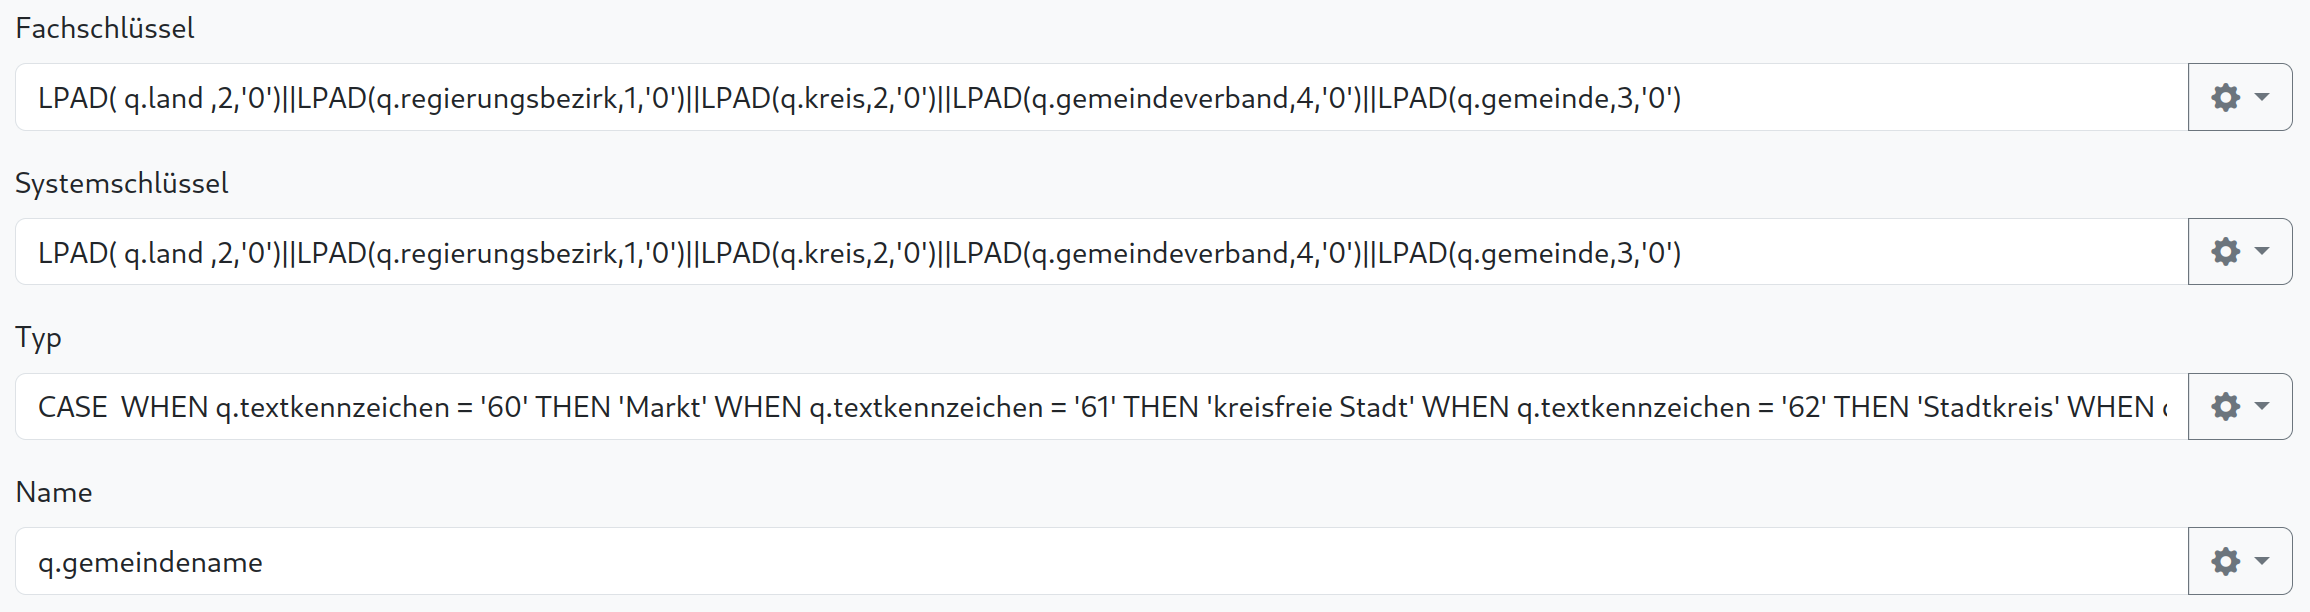
\includegraphics[width=.95\textwidth]{assets/conversion-gemeinde.png}
  \caption{Auszug aus der Konvertierungsdefinition für die Objektklasse "Gemeinde" im aktuellen Editor für Konvertierungen.}
  \label{fig:conversion-gemeinde}
\end{figure}

Der aktuelle Editor für Konvertierungen besteht aus Textfeldern, in denen Auszüge von \ac{sql}-Befehlen eingegeben werden können. Ein Beispiel dafür ist in Abbildung \ref{fig:conversion-gemeinde} gegeben. Für jedes Attribut wird dies dann in einem \texttt{SELECT}-Befehl eingesetzt. Diese Herangehensweise ist äußerst flexibel, weißt jedoch in der Benutzung einige Usability-Probleme auf: Erstens sind die Ausgangsdaten nicht innerhalb des Editors dokumentiert.\todo[noline]{mehr auf bild eingehen?} Die Benutzer:innen müssen somit immer nachschlagen, welche Werte sie eintragen können. Das manuelle Eintippen birgt außerdem die Gefahr, sowohl Tippfehler als auch Fehler im \ac{sql}-Syntax zu verursachen. Auch die inhaltliche Sinnhaftigkeit der Befehle wird nicht sichergestellt, und Nutzer:innen, die nicht vertraut mit SQL sind, benötigen aufwendige Einführungen und können komplexe Aufgaben schlechter bewältigen. \todo[noline]{oh oh alles nicht belegt}

Der entwickelte Editor sollte in Sachen Nutzbarkeit eine Verbesserung gegenüber der aktuellen Lösung darstellen. Es sollte weniger Nachschlagearbeit nötig sein, weniger Tippfehler auftreten und auch für Personen, die keinen technischen Hintergrund oder \ac{sql}-Vorkenntnisse besitzen, nutzbar sein.

Zusammenfassend können folgende Ziele formuliert werden:
\begin{itemize}
  \item Entwicklung eines Editors für Konvertierungen und Szenarien.
  \item Der Editor soll häufiges Nachschlagen verhindern.
  \item Der Editor soll Tippfehlern vorbeugen.
  \item Der Editor soll auch ohne \ac{sql}-Kenntnisse bedienbar sein.
\end{itemize}
